% This file was created with tikzplotlib v0.10.1.post5.
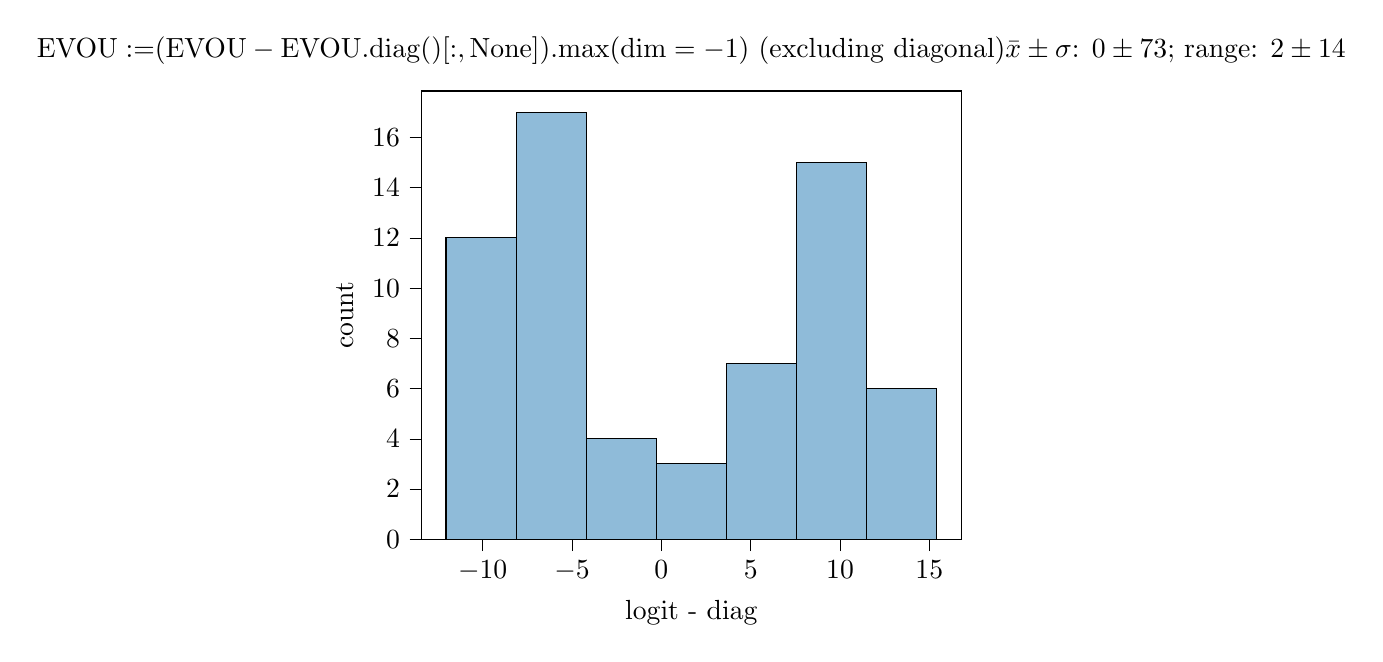
\begin{tikzpicture}

\definecolor{darkgray176}{RGB}{176,176,176}
\definecolor{steelblue31119180}{RGB}{31,119,180}

\begin{axis}[
tick align=outside,
tick pos=left,
title={\(\displaystyle \mathrm{EVOU} := \WE \WV \WO\WU \)\\
\(\displaystyle (\mathrm{EVOU} - \mathrm{EVOU}\mathrm{.diag}()[:,\mathrm{None}])\mathrm{.max}(\mathrm{dim}=-1)\) (excluding diagonal)\\
\(\displaystyle \bar{x}\pm\sigma\): \(\displaystyle 0 \pm 73\); range: \(\displaystyle 2 \pm 14\)},
x grid style={darkgray176},
xlabel={logit - diag},
xmin=-13.4269836425781, xmax=16.7784698486328,
xtick style={color=black},
xtick={-15,-10,-5,0,5,10,15,20},
xticklabels={
  \(\displaystyle {\ensuremath{-}15}\),
  \(\displaystyle {\ensuremath{-}10}\),
  \(\displaystyle {\ensuremath{-}5}\),
  \(\displaystyle {0}\),
  \(\displaystyle {5}\),
  \(\displaystyle {10}\),
  \(\displaystyle {15}\),
  \(\displaystyle {20}\)
},
y grid style={darkgray176},
ylabel={count},
ymin=0, ymax=17.85,
ytick style={color=black},
ytick={0,2,4,6,8,10,12,14,16,18},
yticklabels={
  \(\displaystyle {0}\),
  \(\displaystyle {2}\),
  \(\displaystyle {4}\),
  \(\displaystyle {6}\),
  \(\displaystyle {8}\),
  \(\displaystyle {10}\),
  \(\displaystyle {12}\),
  \(\displaystyle {14}\),
  \(\displaystyle {16}\),
  \(\displaystyle {18}\)
}
]
\draw[draw=black,fill=steelblue31119180,fill opacity=0.5] (axis cs:-12.0540084838867,0) rectangle (axis cs:-8.13122231619699,12);
\draw[draw=black,fill=steelblue31119180,fill opacity=0.5] (axis cs:-8.13122231619699,0) rectangle (axis cs:-4.20843614850725,17);
\draw[draw=black,fill=steelblue31119180,fill opacity=0.5] (axis cs:-4.20843614850725,0) rectangle (axis cs:-0.285649980817522,4);
\draw[draw=black,fill=steelblue31119180,fill opacity=0.5] (axis cs:-0.285649980817523,0) rectangle (axis cs:3.63713618687221,3);
\draw[draw=black,fill=steelblue31119180,fill opacity=0.5] (axis cs:3.63713618687221,0) rectangle (axis cs:7.55992235456194,7);
\draw[draw=black,fill=steelblue31119180,fill opacity=0.5] (axis cs:7.55992235456194,0) rectangle (axis cs:11.4827085222517,15);
\draw[draw=black,fill=steelblue31119180,fill opacity=0.5] (axis cs:11.4827085222517,0) rectangle (axis cs:15.4054946899414,6);
\end{axis}

\end{tikzpicture}
